\documentclass[a4paper,12pt]{article}

% Kodowanie i język
\usepackage[utf8]{inputenc}
\usepackage[T1]{fontenc}
\usepackage[polish]{babel}
\usepackage{lmodern}  % nowoczesna czcionka

% Bibliografia
\usepackage[
sorting=none
]{biblatex} %Imports biblatex package
\addbibresource{doc.bib} %Import the bibliography file

% Ustawienia strony
\usepackage{geometry}
\geometry{a4paper, margin=2.5cm}

% Pakiety graficzne i multimedialne
\usepackage{graphicx}
\usepackage{float}
\usepackage{caption}
\usepackage{subcaption}
\usepackage{tabularx}

% Pakiety dla kodu źródłowego
\usepackage{listings}
\usepackage{xcolor}
\lstset{%
  language=Java,                % język programowania (dostosuj w razie potrzeby)
  basicstyle=\footnotesize\ttfamily,
  numbers=left,
  numberstyle=\tiny,
  stepnumber=1,
  numbersep=5pt,
  backgroundcolor=\color{white},
  showspaces=false,
  showstringspaces=false,
  showtabs=false,
  frame=single,
  tabsize=2,
  captionpos=b,
  breaklines=true,
  breakatwhitespace=false,
  escapeinside={\%*}{*)}
}

% Matematyka
\usepackage{amsmath, amssymb}

% Nagłówki i stopki
\usepackage{fancyhdr}
\pagestyle{fancy}
\fancyhf{}
\fancyfoot[L]{
\includegraphics[height=0.8cm]{assets/media/image1.png}}
\fancyfoot[C]{\thepage}
\renewcommand{\headrulewidth}{0pt}
\renewcommand{\footrulewidth}{0.5pt}


% Odnośniki
\usepackage{hyperref}
\hypersetup{
    colorlinks=false,
    linkcolor=blue,
    pdftitle={Dokumentacja Techniczna: Absolute Casino},
}

% Dodatkowe pakiety
\usepackage{enumitem}
\usepackage{longtable}
\usepackage{booktabs}
\usepackage{tikz}
\usepackage{pgfplots}
\usepackage{titlesec}
%\usepackage{indentfirst}

\pgfplotsset{compat=1.18}
\begin{document}


% Strona tytułowa
\begin{titlepage}
    \begin{center}
        \vspace*{2cm}
        
\includegraphics[width=0.4\textwidth]{assets/media/image1.png}
        \vspace{1cm}

        {\Huge \bfseries Dokumentacja Techniczna \par}
        \vspace{1cm}
        {\Large Projekt kasyna internetowego "Absolute Casino"\par}
        \vspace{1cm}
        {\Large Autorzy: Mateusz Kroplewski, Aleksander Olkowicz, Paweł Wójcik, Kacper Araszkiewicz\par}
        \vspace{1cm}
        {\Large Data: \today\par}
        \vspace{1cm}
    \end{center}
\end{titlepage}

% Spis treści
\tableofcontents
\newpage

\section{Opis problemu}

Symulator kasyna jest aplikacją umożliwiającą użytkownikowi rozgrywkę w dwóch grach karcianych oraz na dwóch automatach typu slot. Projekt ma na celu stworzenie realistycznego środowiska hazardowego, które może być wykorzystywane do celów edukacyjnych, rozrywkowych oraz badawczych. Celem projektu jest proof of concept systemu kasynowego, który pozwoli na testowanie różnych strategii gry oraz analizowanie mechanizmów losowości i prawdopodobieństwa.

\subsection{Porównanie dostępnych rozwiązań}

Na rynku istnieje wiele symulatorów kasynowych, jednak różnią się one zakresem funkcjonalności oraz poziomem realizmu. Część z nich koncentruje się na rozrywce, oferując uproszczone wersje gier w których znacznie łatwiej jest wygrać, natomiast inne mają charakter bardziej analityczny, umożliwiając badanie strategii graczy. W ramach naszej pracy analizujemy dostępne rozwiązania pod kątem mechaniki gier, generowania losowości oraz systemów nagradzania. Wszystkie zastosowane mechaniki w naszych grach są oparte na realnym prawdopodobieństwie występującym w kasynach.

\subsection{Możliwości zastosowania praktycznego}

Symulator kasyna może być wykorzystywany do różnych celów, takich jak:
\begin{itemize}
    \item Nauka zasad i strategii gier hazardowych bez ryzyka finansowego,
    \item Testowanie algorytmów generowania liczb losowych i mechanizmów fair play,
    \item Symulacja różnych modeli kasynowych w celu analizy ich rentowności,
    \item Narzędzie badawcze do analizowania zachowań graczy i skuteczności strategii.
    \item Potencjalne użycie gier w prawdziwym kasynie po uzyskaniu koncesji.
\end{itemize}

\subsection{Aspekt badawczy projektu}

Badania związane z projektem skupiają się na analizie mechanizmów losowości, strategii graczy oraz psychologii hazardu. Istotnym elementem jest również ocena wpływu symulowanych warunków kasynowych na podejmowane decyzje oraz badanie efektywności różnych strategii gry. Podczas prezentacji naszego projektu mogliśmy również zauważyć jakie gry preferują gracze i jakie aspekty psychologii hazardu oraz wizualne wzbudzają większe zainteresowanie.


\newpage
\section{Projekt i analiza}
\subsection{Aktorzy i przypadki użycia}

W tej sekcji przedstawiony zostanie diagram przypadków użycia, który ilustruje interakcje pomiędzy użytkownikami a systemem. Diagram przypadków użycia jest narzędziem modelowania w UML, używanym do przedstawienia funkcjonalności systemu z perspektywy użytkowników. Składa się z aktorów, reprezentujących użytkowników lub inne systemy, oraz przypadków użycia, czyli konkretnych funkcji dostępnych w systemie. Aktorzy w diagramie przypadków użycia to elementy zewnętrzne wobec systemu, które wchodzą z nim w interakcję. Mogą to być osoby, inne systemy lub urządzenia, które inicjują określone działania lub reagują na operacje systemu. Każdy aktor pełni określoną rolę w systemie i posiada dostęp do wybranych przypadków użycia.

\subsubsection*{Aktorzy}

\begin{enumerate}
\def\labelenumi{\arabic{enumi}.}
\item
  \textbf{Gracz} -- użytkownik końcowy, który loguje się do systemu,
  wpłaca środki, gra w gry hazardowe i wypłaca wygrane.
\item
  \textbf{Administrator} -- osoba zarządzająca systemem, moderująca
  użytkowników, monitorująca transakcje oraz ustawienia gier.
\item
  \textbf{System Płatności} -- system obsługujący wpłaty i wypłaty
  środków.
\item
  \textbf{System bonusów} -- moduł odpowiedzialny za przydzielanie
  bonusów do gier slotowych.
\item
  \textbf{System Losujący (RNG -- Random Number Generator \cite{rng})} -- moduł
  odpowiedzialny za losowe wyniki gier.
\end{enumerate}

\subsubsection*{Przypadki Użycia}

\begin{enumerate}
\def\labelenumi{\arabic{enumi}.}
\item
  \textbf{Rejestracja nowego gracza} -- Gracz zakłada konto, podając
  wymagane dane i potwierdzając tożsamość.
\item
  \textbf{Logowanie gracza} -- Gracz loguje się do systemu za pomocą
  loginu i hasła.
\item
  \textbf{Wpłata środków} -- Gracz dodaje środki na swoje konto poprzez
  system płatności.
\item
  \textbf{Wybór gry} -- Gracz wybiera pomiędzy grami slotowymi a
  karcianymi.
\item
  \textbf{Rozgrywka} -- Gracz uczestniczy w grze, system losuje wyniki.
\item
  \textbf{Odbiór wygranej} -- Gracz otrzymuje wygrane środki na konto.
\item
  \textbf{Konfiguracja gier} -- Administrator dostosowuje ustawienia
  gier.
\item
  \textbf{Blokowanie użytkownika} -- Administrator może zablokować konto
  gracza w przypadku naruszenia regulaminu.
\end{enumerate}

\begin{figure}[H]
  \centering
  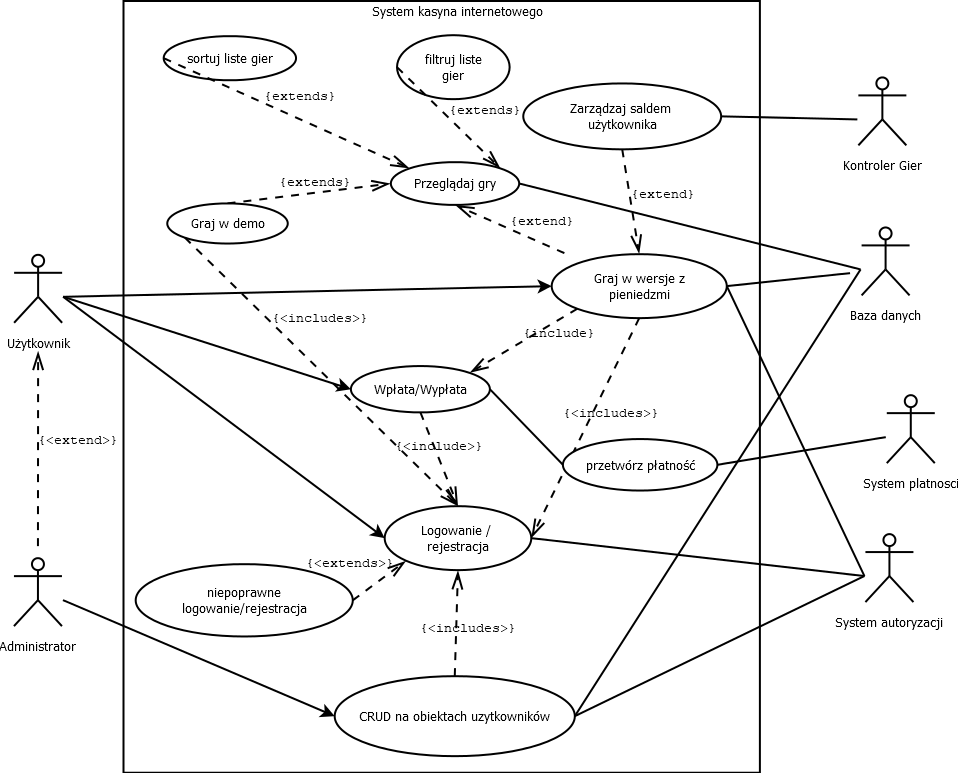
\includegraphics[width=14cm]{assets/media/pu.png}
  \caption{Diagram przypadków użycia [stworzony w programie dia]}
  \label{fig:control}
\end{figure}



\subsection{Wymagania funkcjonalne}
Wymagania funkcjonalne to określone działania i funkcje, jakie system ma realizować. Opisują, co system ma robić, np. rejestracja użytkownika, logowanie, przetwarzanie płatności czy generowanie wyników gry. Poniżej wymagania funkcjonalne projektu:

\begin{enumerate}
\def\labelenumi{\arabic{enumi}.}
\item
  \textbf{Rejestracja i logowanie}:

  \begin{itemize}
  \item
    Możliwość rejestracji nowych użytkowników.
  \item
    Weryfikacja tożsamości graczy za pomocą tokenu \textbf{JWT} \cite{jwt}.
  \end{itemize}
\item
  \textbf{Obsługa wpłat i wypłat}:

  \begin{itemize}
  \item
    Symulacja systemu wpłat.
  \end{itemize}
\item
  \textbf{Gry hazardowe}:

  \begin{itemize}
  \item
    Implementacja gier slotowych i karcianych.
  \item
    Zastosowanie algorytmu RNG dla uczciwości losowania.
  \item
    Możliwość ustawiania limitów zakładów dla danej gry.
  \item
    System bonusów
  \end{itemize}
\item
  \textbf{Bezpieczeństwo i zgodność}:

  \begin{itemize}
  \item
    Mechanizmy ochrony przed nadużyciami implementacji gier.
  \end{itemize}
\item
  \textbf{Zarządzanie użytkownikami}:

  \begin{itemize}
  \item
    Możliwość blokowania kont naruszających regulamin.
  \item
    Historia transakcji i gier dostępna dla administratora.
  \end{itemize}
\item
  \textbf{Interfejs użytkownika}:

  \begin{itemize}
  \item
    Responsywny interfejs dostępny na komputery i urządzenia mobilne.
  \item
    Czytelne statystyki wygranych i przegranych.
  \end{itemize}
\end{enumerate}

\textbf{Wymagania niefunkcjonalne}

\begin{enumerate}
\def\labelenumi{\arabic{enumi}.}
\item
  \textbf{Wydajność}:
  \begin{itemize}
  \item
    Czas odpowiedzi systemu nie powinien przekraczać 1 sekundy.
  \end{itemize}
\item
  \textbf{Bezpieczeństwo}:
  \begin{itemize}
  \item
    Szyfrowanie danych użytkowników.
  \end{itemize}
\item
  \textbf{Skalowalność}:
  \begin{itemize}
  \item
    Możliwość dodawania nowych gier bez konieczności modyfikacji całego
    systemu.
  \end{itemize}
\item
  \textbf{Dostępność}:
  \begin{itemize}
  \item
    System dostępny 24/7.
  \item
    Maksymalny czas niedostępności nie przekracza 5 minut miesięcznie.
  \end{itemize}
\end{enumerate}

\subsection{Diagramy klas}

W tej sekcji przedstawione zostaną diagramy klas dla systemu gier, które ilustrują strukturę systemu i relacje między jego elementami. Diagram klas to narzędzie modelowania w UML, używane do przedstawienia struktur danych w systemie. Składa się z klas, atrybutów, metod oraz powiązań między klasami, takich jak dziedziczenie, kompozycja czy asocjacja.

\begin{figure}[H]
  \centering
  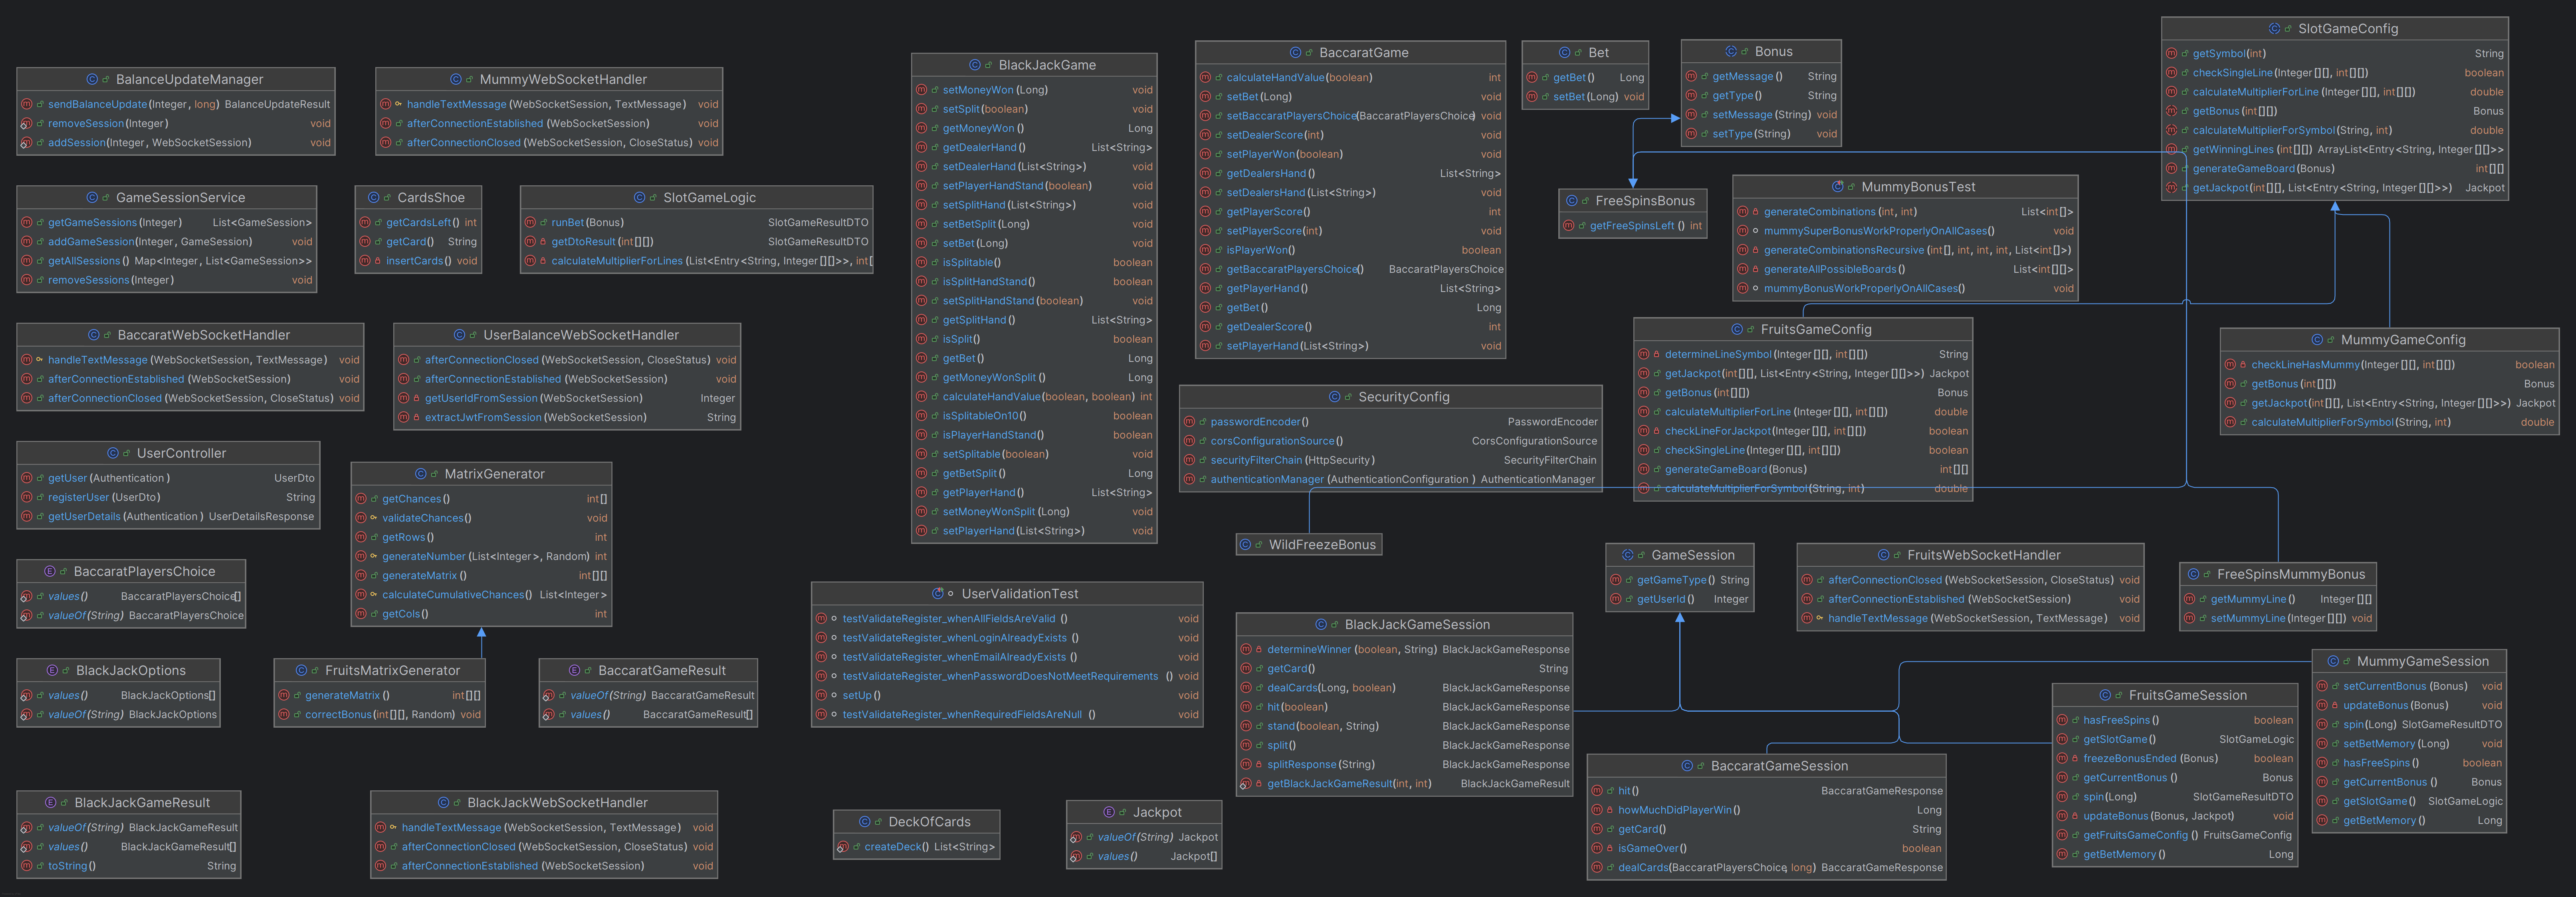
\includegraphics[width=14cm]{assets/media/control.png}
  \caption{Diagram klas - Control [wygenerowane za pomocą IntelijIdea]}
  \label{fig:control}
\end{figure}

\begin{figure}[H]
  \centering
  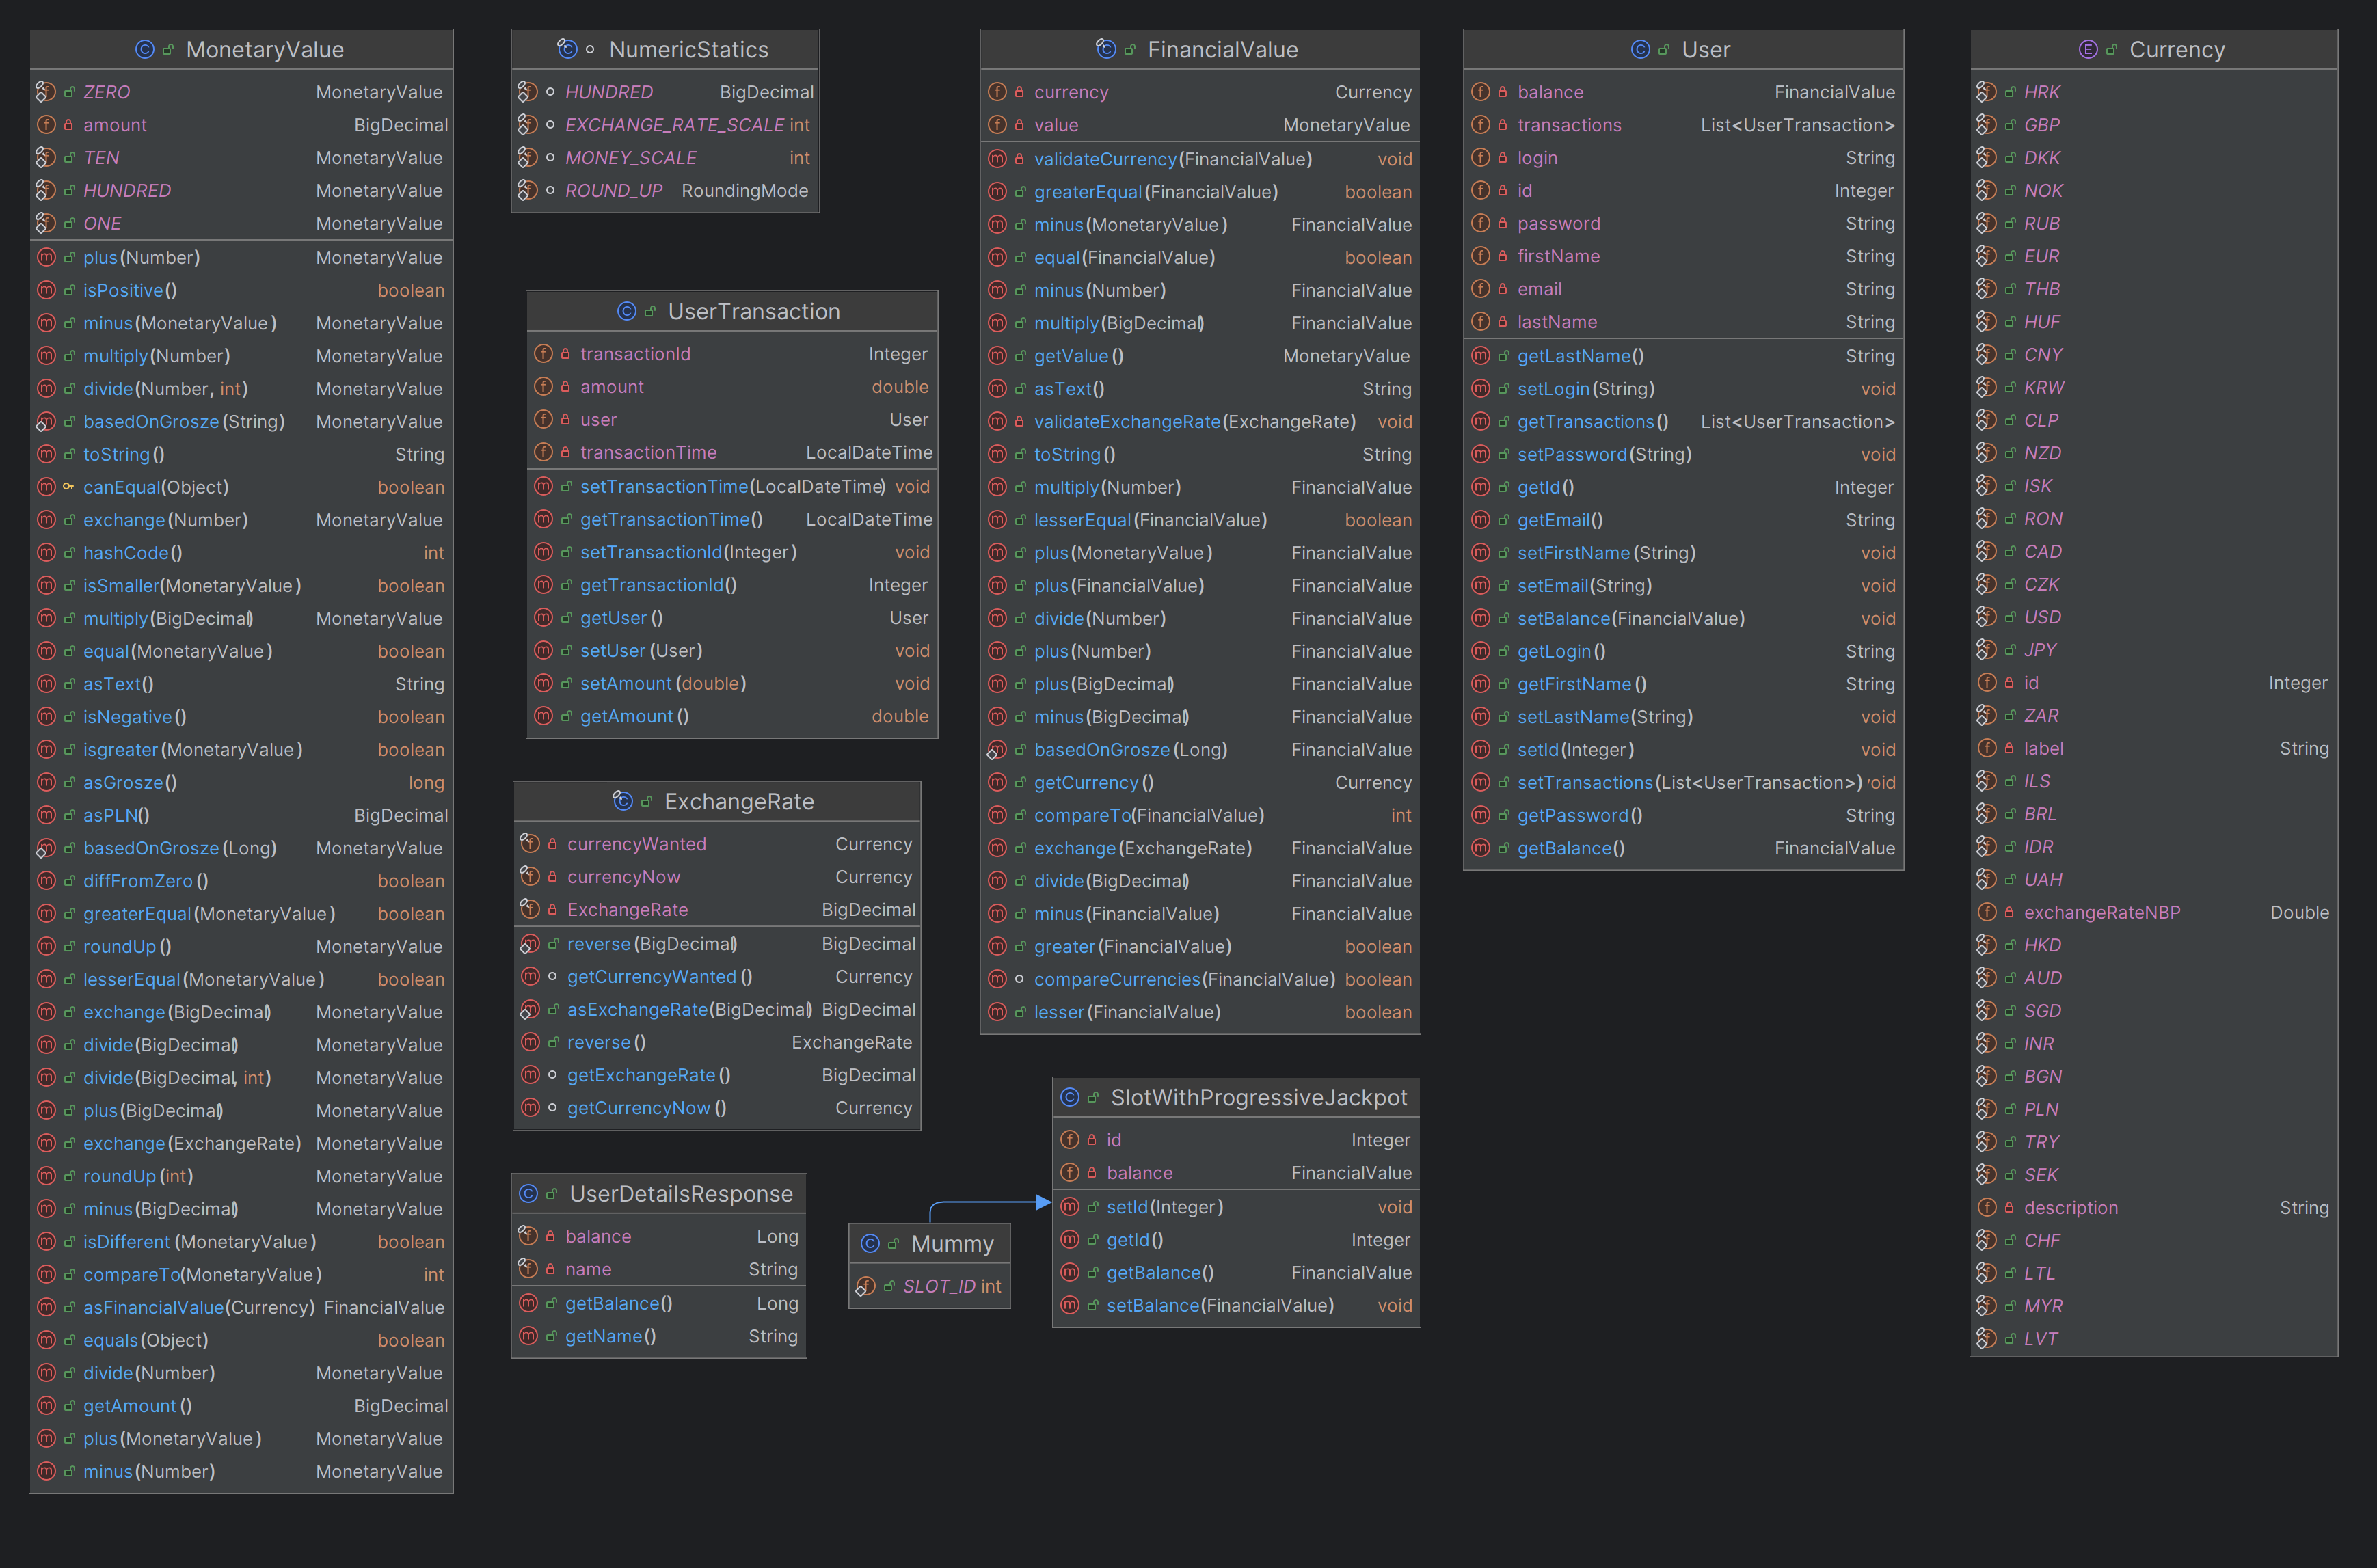
\includegraphics[width=14cm]{assets/media/model.png}
  \caption{Diagram klas - Model [wygenerowane za pomocą IntelijIdea]}
  \label{fig:model}
\end{figure}

\begin{figure}[H]
  \centering
  
\includegraphics[width=14cm]{assets/media/repository.png}
  \caption{Diagram klas - Repository [wygenerowane za pomocą IntelijIdea]}
  \label{fig:repository}
\end{figure}

\begin{figure}[H]
  \centering
  
\includegraphics[width=14cm]{assets/media/view.png}
  \caption{Diagram klas - View [wygenerowane za pomocą IntelijIdea]}
  \label{fig:view}
\end{figure}

\subsection{Diagram modelu danych}
W tej sekcji przedstawiony zostanie diagram modelu danych dla systemu gier, który ilustruje strukturę przechowywania danych w systemie. Diagram modelu danych to schemat przedstawiający organizację danych w systemie, w tym tabele, atrybuty oraz relacje między nimi. Służy do zaprojektowania logicznej i fizycznej struktury bazy danych, pokazując, jak dane są przechowywane i powiązane.

\begin{figure}[H]
  \centering
  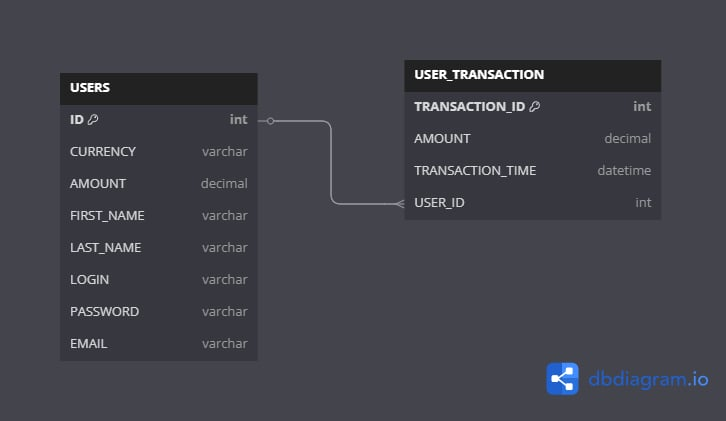
\includegraphics[width=14cm]{assets/media/data_model.png}
  \caption{Diagram modelu danych [wygenerowane za pomocą DiagramDB.io]}
  \label{fig:data_model}
\end{figure}

\subsection{Projekt interfejsu użytkownika}
Interfejs użytkownika odgrywa kluczową rolę w doświadczeniu użytkownika każdej aplikacji internetowej. W przypadku platform kasynowych, design powinien być nie tylko estetyczny, ale także funkcjonalny i intuicyjny. Poniżej opisane zostały kluczowe aspekty interfejsu oraz załączone rysunki z projektami graficznymi głównych obszarów strony.

\subsubsection*{Schemat kolorów}
Interfejs wykorzystuje dominujące ciemne odcienie granatu i czerni, co nadaje mu elegancki i ekskluzywny wygląd. Kluczowe akcenty kolorystyczne:
\begin{itemize}
    \item Złote elementy (logo, nagłówki, obramowania) podkreślają luksusowy charakter strony oraz nawiązują do złota.
    \item Jaskrawe kolory w grafikach gier tworzą kontrast i przyciągają uwagę użytkownika.
\end{itemize}

\subsubsection*{Minimalistyczny design}
Układ strony jest przejrzysty i uporządkowany:
\begin{itemize}
    \item Prosty pasek nawigacyjny w prawym górnym rogu zawiera elementy: FAQ, Regulamin, oraz przyciski logowania i rejestracji.
    \item Ograniczona liczba elementów na stronie zapewnia estetyczny wygląd bez zbędnego przeciążenia wizualnego.
\end{itemize}

\subsubsection*{Struktura treści}
Strona jest podzielona na dwie główne sekcje:
\begin{itemize}
    \item \textbf{Sloty} – zawiera gry na automaty: \textit{Mummy} i \textit{Fruitogedon}.
    \item \textbf{Gry Karciane} – obejmuje gry stołowe: \textit{Blackjack} i \textit{Baccarat}.
\end{itemize}
Każda gra jest przedstawiona w formie grafiki zachęcającej do kliknięcia.


\begin{figure}[H]
  \centering
  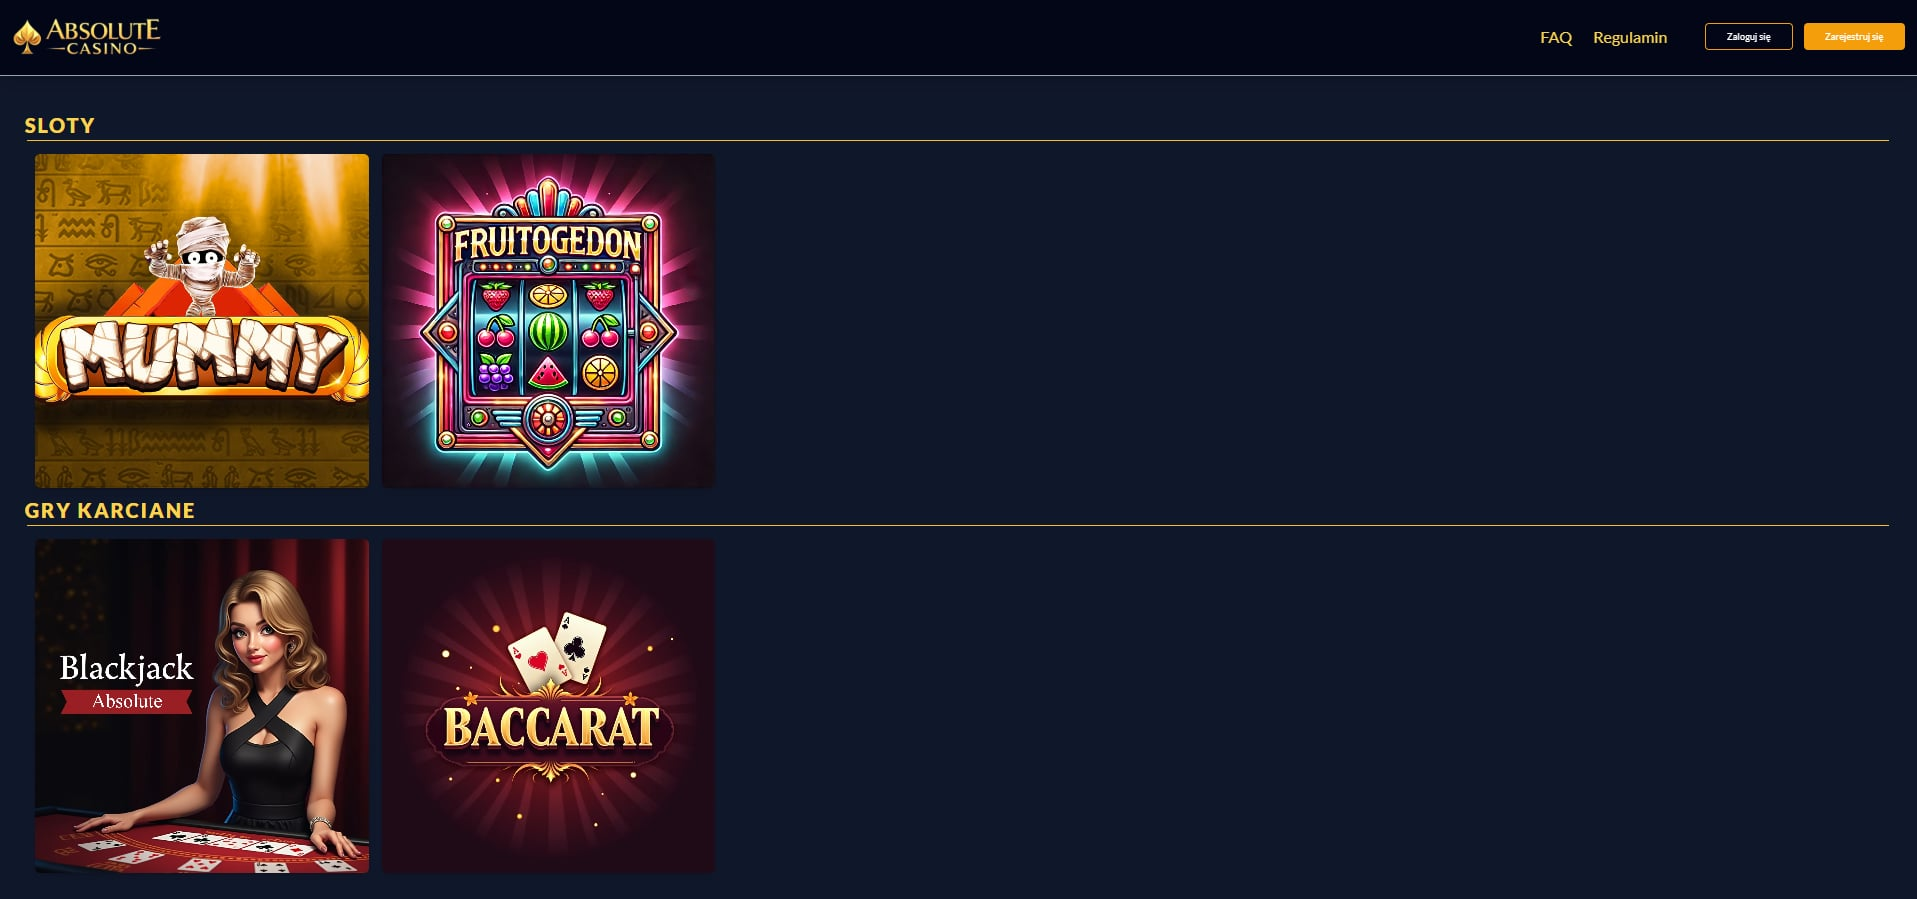
\includegraphics[width=14cm]{assets/media/MainPage.png}
  \caption{Strona główna [opracowanie własne}
  \label{fig:MainPage}
\end{figure}

\begin{figure}[H]
  \centering
  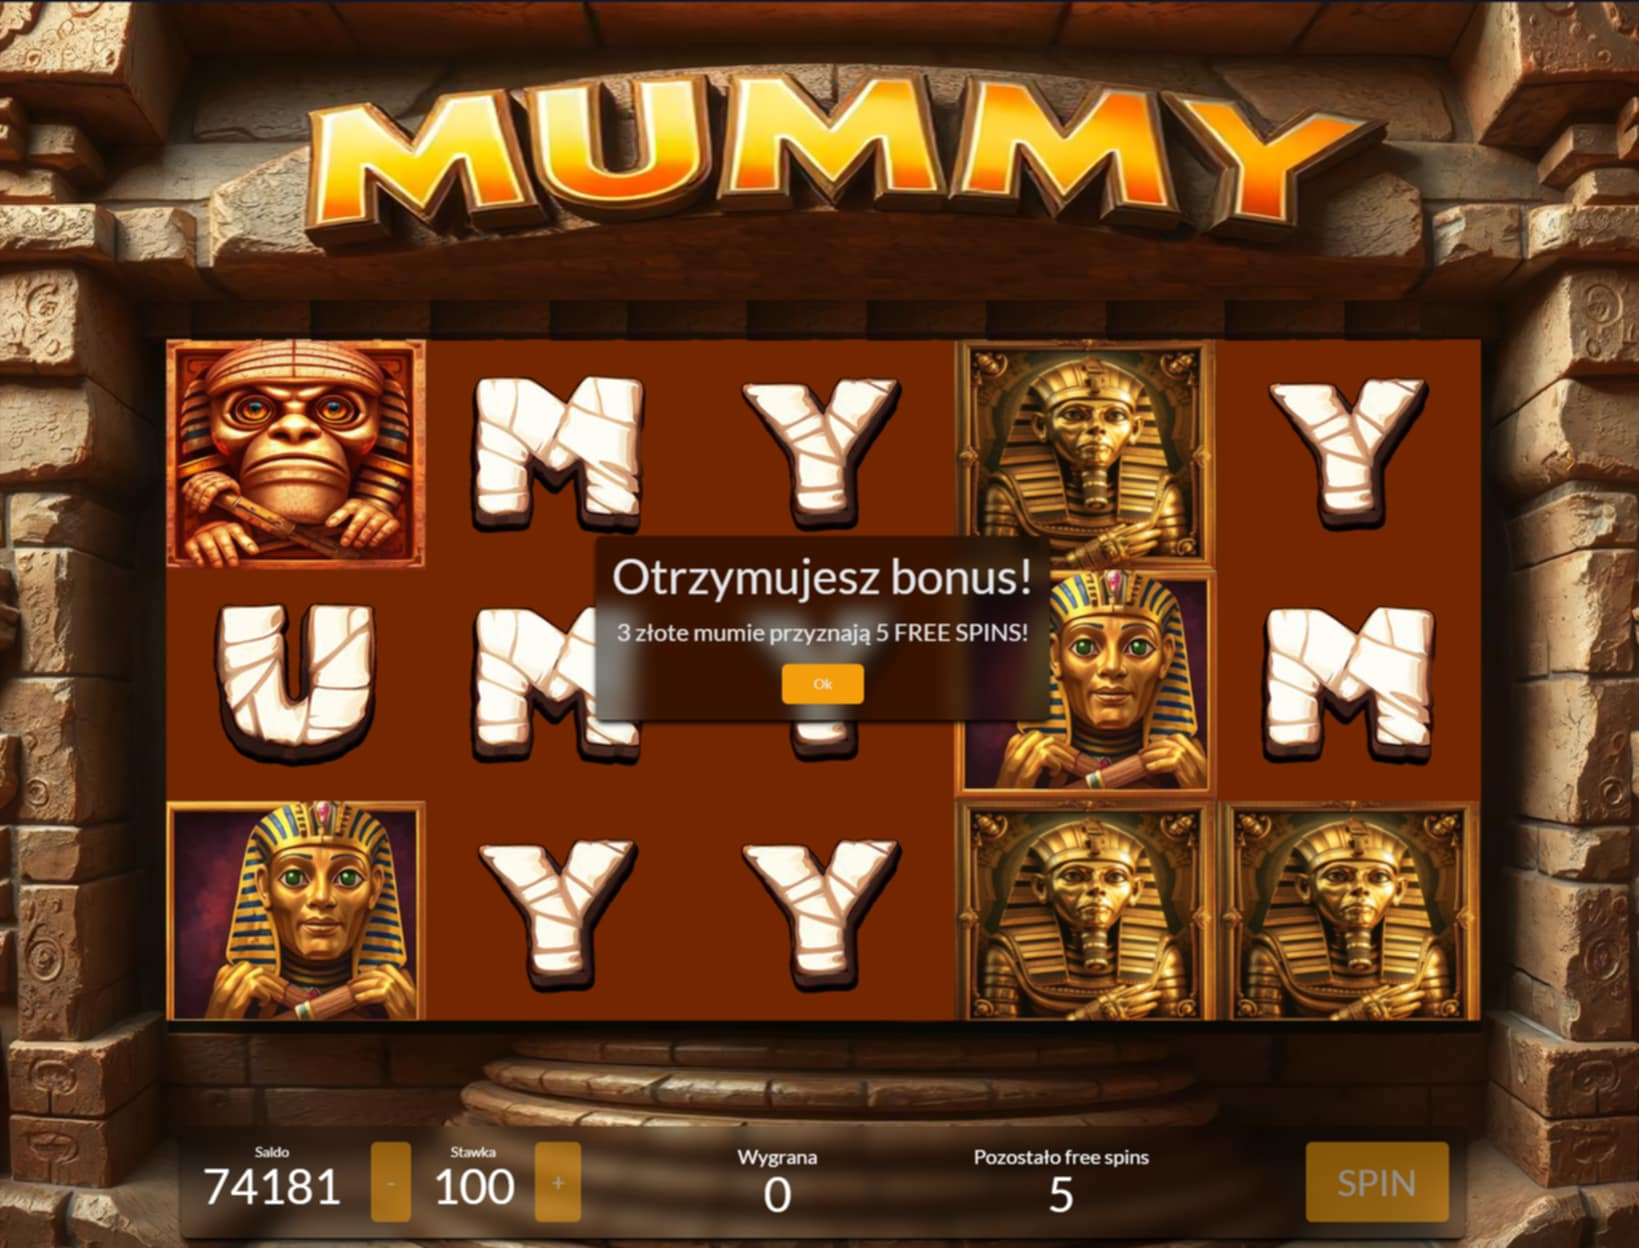
\includegraphics[width=14cm]{assets/media/Mummy.png}
  \caption{Gra typu slot - Mummy [opracowanie własne}
  \label{fig:Mummy}
\end{figure}

\begin{figure}[H]
  \centering
  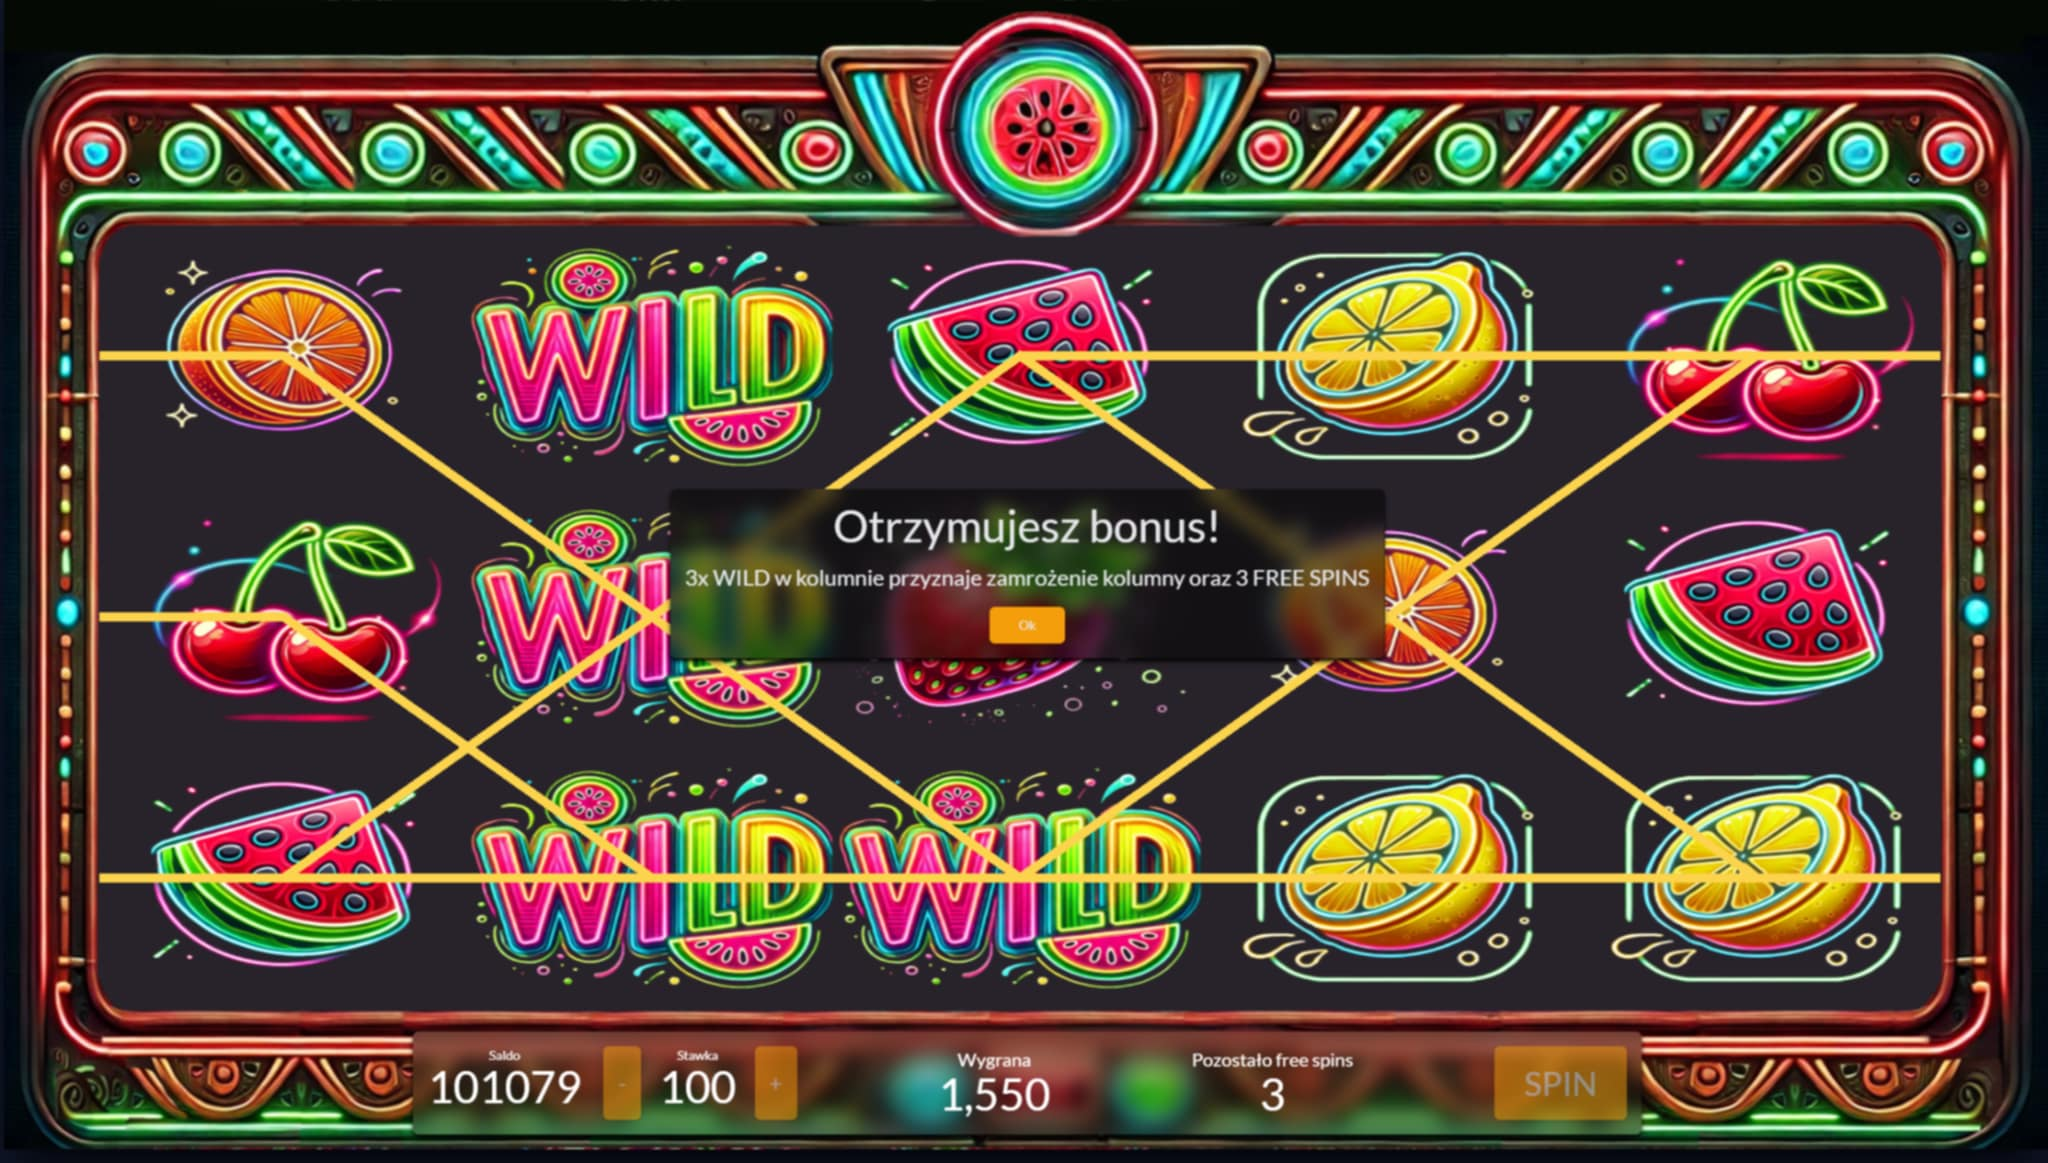
\includegraphics[width=14cm]{assets/media/Fruitogedon.png}
  \caption{Gra typu slot - Fruitogedon [opracowanie własne]}
  \label{fig:Fruitogedon}
\end{figure}

\begin{figure}[H]
  \centering
  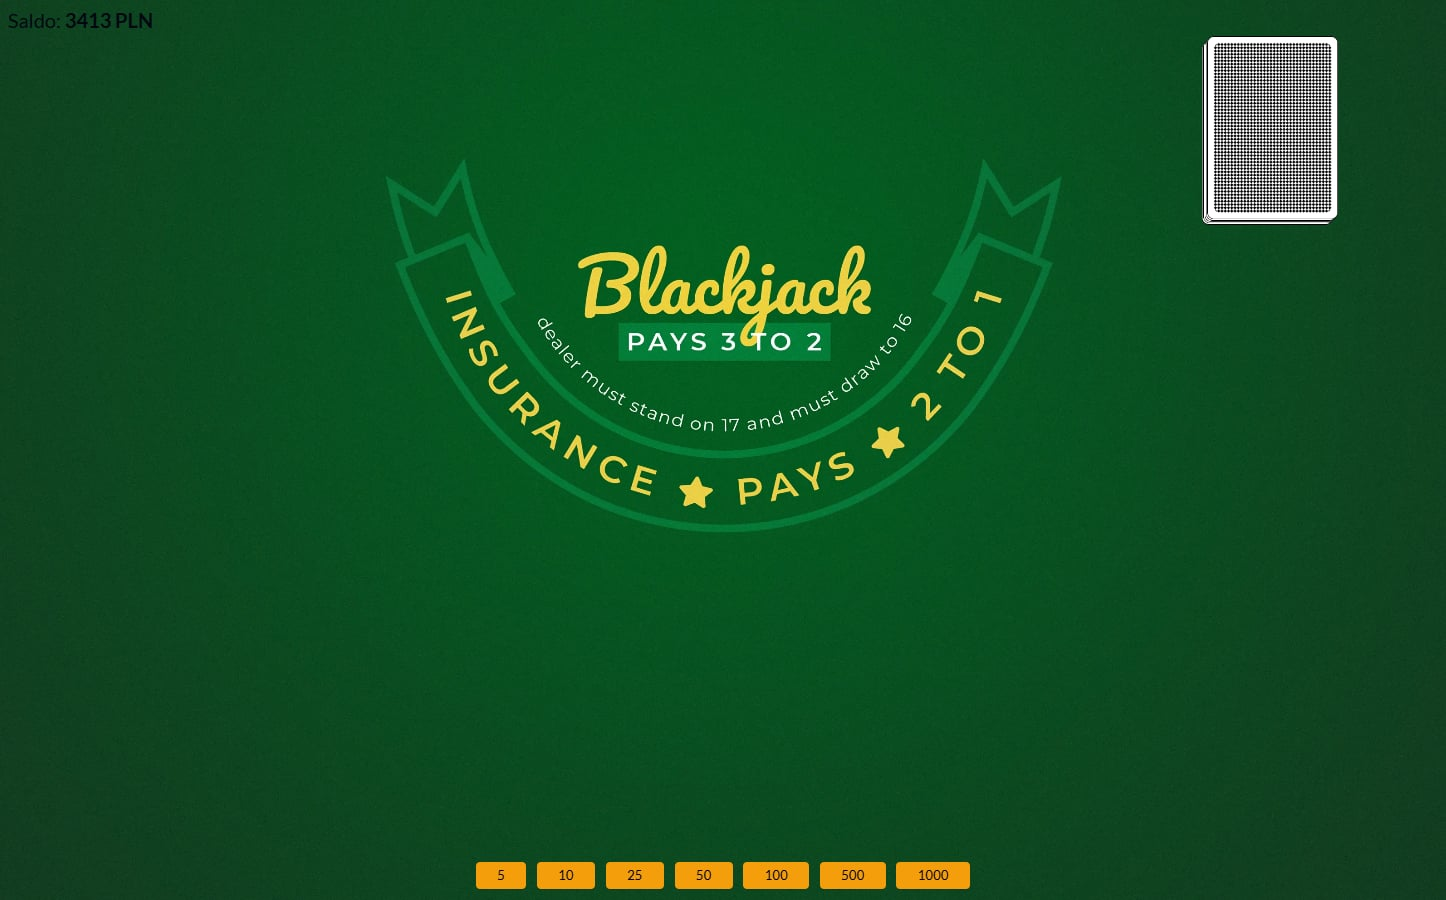
\includegraphics[width=14cm]{assets/media/Blackjack.png}
  \caption{Gra karciana - Blackjack [opracowanie własne}
  \label{fig:Blackjack}
\end{figure}

\begin{figure}[H]
  \centering
  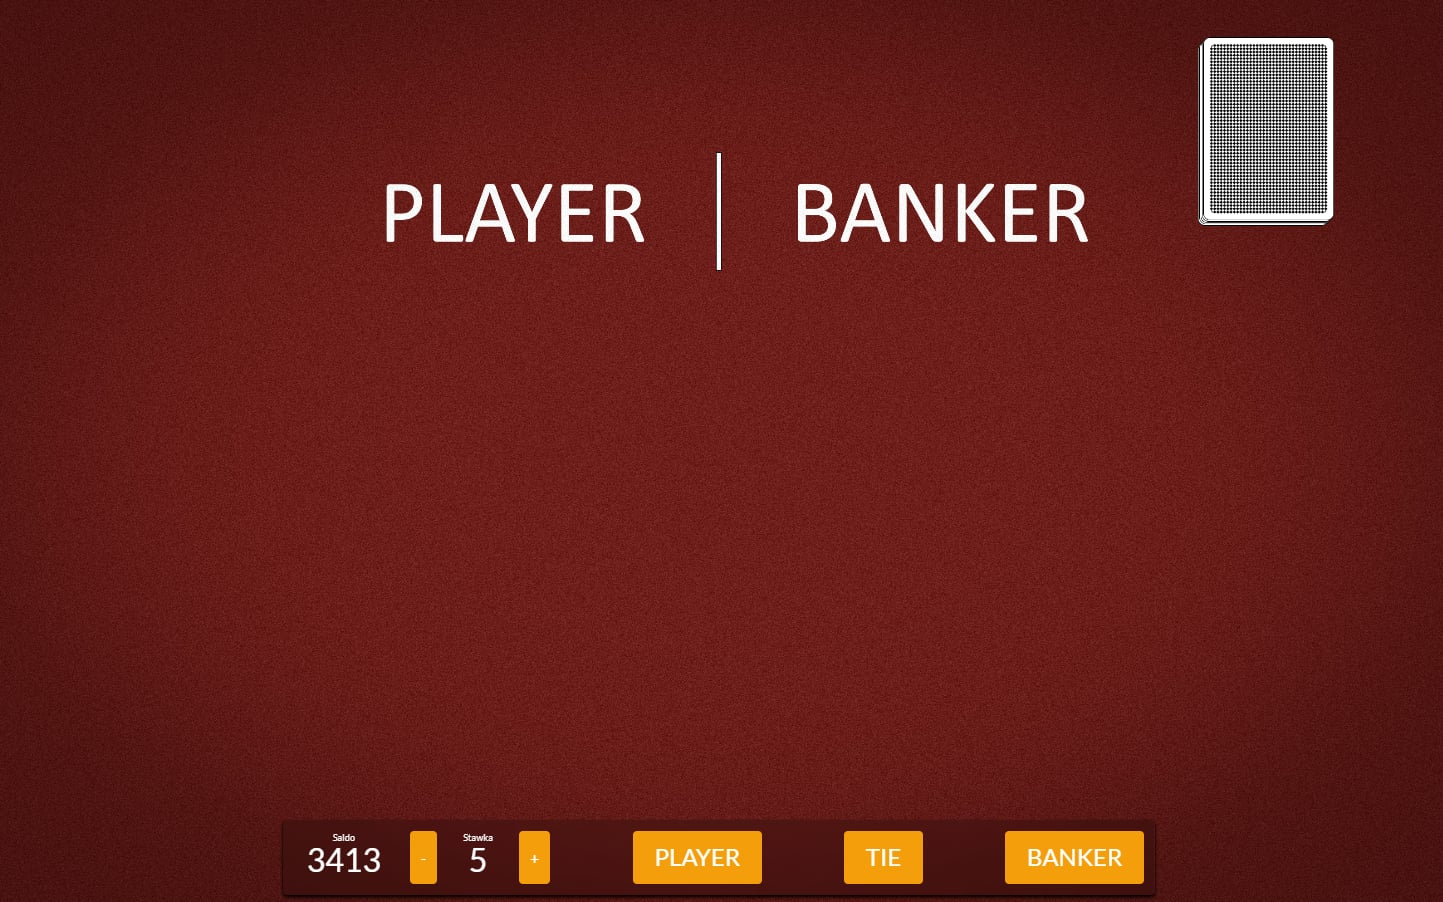
\includegraphics[width=14cm]{assets/media/Baccarat.png}
  \caption{Gra karciana - Baccarat [opracowanie własne}
  \label{fig:Baccarat}
\end{figure}

\newpage
\section{Implementacja}

\subsection{Architektura rozwiązania}
Projekt "Absolute Casino" został zaprojektowany w oparciu o podejście wielowarstwowe, co pozwala na logiczne oddzielenie poszczególnych funkcjonalności. W skrócie, nasza architektura składa się z następujących elementów:
\begin{itemize}[noitemsep]
    \item \textbf{Backend:}  
    Nasz serwer napisany jest w Javie przy użyciu Spring Boot, co umożliwia szybkie i elastyczne tworzenie aplikacji. Zaimplementowaliśmy własny mechanizm autentykacji, dzięki któremu mamy pełną kontrolę nad logowaniem i zarządzaniem sesjami użytkowników. Dodatkowo, backend obsługuje komunikację przez WebSockety – jeden kanał jest wykorzystywany do dynamicznych rozgrywek, a drugi do aktualizacji stanu konta.
    
    \item \textbf{Frontend:}  
    Interfejs użytkownika zbudowany został w React. Dzięki wykorzystaniu nowoczesnych bibliotek, udało nam się stworzyć responsywną i skalowalną aplikację. Umożliwia ona płynne przechodzenie między widokami, dynamiczne renderowanie gier oraz animacje, co jest kluczowe przy obsłudze interaktywnego środowiska kasyna.
    
    \item \textbf{Baza danych:}  
    Podczas prac deweloperskich korzystamy z lekkiej bazy H2, co znacząco ułatwia testowanie i rozwój aplikacji. W produkcji planujemy użyć PostgreSQL – system ten zapewnia stabilność i skalowalność, które są niezbędne przy dużej liczbie użytkowników.
    
    \item \textbf{Komunikacja w czasie rzeczywistym:}  
    Cała komunikacja między frontendem a backendem odbywa się przez WebSockety. To podejście umożliwia natychmiastowe przesyłanie wyników gier oraz szybką aktualizację stanu konta użytkownika.
\end{itemize}

\subsection{Użyte technologie}
W trakcie tworzenia "Absolute Casino" zdecydowaliśmy się na zestaw nowoczesnych narzędzi, które ułatwiają zarówno rozwój aplikacji, jak i utrzymanie jej wysokiej wydajności. Oto, z czego korzystamy:
\begin{itemize}[noitemsep]
    \item \textbf{Backend:}
    \begin{itemize}[noitemsep]
        \item \textbf{Java + Spring Boot:} Główny framework, który umożliwia tworzenie skalowalnych aplikacji.  
        \item \textbf{Własna autentykacja:} Implementacja mechanizmu logowania i zarządzania sesjami, dzięki której zabezpieczamy dostęp do aplikacji.
    \end{itemize}
    
    \item \textbf{Frontend:}
    \begin{itemize}[noitemsep]
        \item \textbf{React \cite{react}:} Podstawa naszego interfejsu, która pozwala na tworzenie interaktywnych i dynamicznych widoków.
        \item \textbf{Tanstack Router \cite{tanstack}:} Ułatwia zarządzanie trasami w aplikacji, dzięki czemu przejścia między widokami są płynne.
        \item \textbf{PixiJS \cite{pixi}:} Biblioteka służąca do renderowania gier – gwarantuje wysoką wydajność i ładną grafikę.
        \item \textbf{Shadcn \cite{shadcn}:} Zestaw komponentów, który przyspiesza tworzenie spójnego i nowoczesnego interfejsu.
        \item \textbf{Tailwind CSS \cite{tailwind}:} Narzędzie do stylizacji, które pozwala szybko tworzyć responsywne i estetyczne strony.
        \item \textbf{React-spring \cite{reactspring}:} Umożliwia tworzenie efektownych animacji, dodając aplikacji dynamiki.
    \end{itemize}
    
    \item \textbf{Baza danych:}
    \begin{itemize}[noitemsep]
        \item \textbf{H2:} Używana lokalnie podczas developmentu, dzięki czemu konfiguracja i testowanie są bardzo proste.
        \item \textbf{PostgreSQL:} Docelowa baza danych w środowisku produkcyjnym, wybrana ze względu na niezawodność i skalowalność.
    \end{itemize}
    
    \item \textbf{Komunikacja:}
    \begin{itemize}[noitemsep]
        \item \textbf{WebSocket \cite{websocket}:} Stosujemy natywną obsługę WebSocketów, co pozwala na efektywną i szybką komunikację w czasie rzeczywistym. Wykorzystywane są dwa kanały – jeden do gier, drugi do aktualizacji stanu konta.
    \end{itemize}
\end{itemize}

Podsumowując, nasz projekt "Absolute Casino" łączy solidne rozwiązania backendowe oparte na Spring Boot z nowoczesnym i dynamicznym frontendem w React. Wykorzystanie wydajnych baz danych oraz natywna obsługa WebSocketów gwarantują, że system jest zarówno elastyczny, jak i gotowy do pracy w środowisku produkcyjnym.


\newpage
\section{Testy}
\subsection{Scenariusz testowania}
W niniejszej sekcji przedstawiono strategię testowania aplikacji, która została podzielona na dwa główne obszary: backend oraz frontend.

\subsubsection{Backend}
Testy backendu obejmują głównie testy jednostkowe \cite{unit_test} skoncentrowane na logice poszczególnych gier, w tym:
\begin{itemize}[noitemsep]
    \item \textbf{Blackjack:} Testy walidują poprawność rozgrywki, obliczania wartości kart, stosowanie zasad gry oraz detekcję wygranej/przegranej.
    \item \textbf{Baccarat:} Testy sprawdzają algorytmy przydzielania punktów, wybór wyniku (gracz, bankier, remis) oraz zgodność z regułami gry.
    \item \textbf{Gry slotowe (Mummy i Fruitogedon):} Testy jednostkowe obejmują walidację algorytmów losujących oraz wyliczania wypłat. Szczególną uwagę poświęcono testowaniu mechanizmów odpowiedzialnych za:
    \begin{itemize}[noitemsep]
        \item \textbf{RTP (Return to Player) \cite{rtp}:} Parametr określający średni procent wypłat w stosunku do postawionych środków. Testy weryfikują, czy obliczenia RTP mieszczą się w oczekiwanych granicach i zapewniają uczciwość rozgrywki.
        \item \textbf{Volatility Index \cite{slot_volatility_variance}:} Wskaźnik zmienności, który definiuje częstotliwość i wielkość wygranych. Testy symulują długotrwałe rozgrywki, aby upewnić się, że rozkład wygranych odpowiada zaprojektowanemu poziomowi ryzyka.
    \end{itemize}
\end{itemize}
W przypadku tego projektu testy jednostkowe backendu są kluczowe, ponieważ gwarantują, że oferowane gry są zgodne z zasadami i regulacjami. Gry karciane operują na sztywnych zasadach co ułatwia ich testowanie, oraz jasne określenie przypadków brzegowych.

Gry slotowe nie mają takich zasad co czyni testowanie ich trudniejszym. Jedyną metodą pozwalająca określenie uczciwości gry jest metoda \textbf{Monte Carlo} \cite{monte_carlo}, tj. rozegranie bardzo dużej ilości gier w celu zdeterminowania wskaźników takich jak RTP.

\subsubsection{Frontend}
Testowanie interfejsu użytkownika dzieli się na dwie grupy:
\begin{itemize}[noitemsep]
    \item \textbf{Testy jednostkowe:} Skupiają się na podstawowych komponentach, takich jak wyświetlanie wartości kart w grze Blackjack. Testy te weryfikują, czy dane są poprawnie renderowane, a logika wyświetlania spełnia oczekiwania projektowe.
    \item \textbf{Testy E2E (End-to-End) \cite{e2e}:} Stanowią większość testów frontendowych. Są to symulacje pełnych scenariuszy rozgrywki, które pozwalają na:
    \begin{itemize}[noitemsep]
        \item Symulację interakcji użytkownika z interfejsem – np. logowanie, wybór gry, podejmowanie zakładów.
        \item Weryfikację przepływu rozgrywki w warunkach zbliżonych do rzeczywistych, gdzie system reaguje na decyzje gracza.
        \item Testowanie komunikacji między frontendem a backendem, co umożliwia wykrycie ewentualnych problemów związanych z synchronizacją danych i odpowiedziami serwera.
    \end{itemize}
\end{itemize}
Testy E2E są niezbędne, ponieważ pozwalają na sprawdzenie, czy wszystkie elementy systemu współpracują ze sobą poprawnie i czy aplikacja jako całość zachowuje się zgodnie z wymaganiami funkcjonalnymi. Jest to jedyny sposób na testowanie jak działa aplikacja z perspektywy użytkownika, czyli poprzez interakcję z interfejsem. Do zaimplementowania testów E2E użyliśmy frameworka \textbf{Playwright} \cite{playwright}, który działa poprzez symulowania realnej przeglądarki. Framework oferuje zautomatyzowane interakcje z interfesjem (np. kliknięcie w przycisk, wypełnienie formularza), lokalizowania elementów na stronie w celu walidacji wyświetlania poprawnych danych, oraz wiele innych funkcji. 

By zagwarantować powtarzalność testów gier, oraz wyeliminować inherencyjną losowość algorytmów na backendzie używamy techniki mockingu. Oznacza to że zastępujemy komunikację z backendem, symulowanymi odpowiedziami, co pozwala nam na testowanie spreparanowanych scenariuszy, w tym przypadków brzegowych.

\subsection{Raport z testów}

\subsubsection{Testy Mummy}
Testy gry Mummy obejmują pełną weryfikację logiki gry po stronie backendu za pomocą testów jednostkowych oraz kompleksowe testy E2E walidujące poprawność wyświetlanych stanów gry oraz interkacje użytkownika. Szczególną uwagę poświęcono testom RTP oraz Volatility gwarantującym sprawiedliwość rozgrywki.

\subsubsection*{Testy jednostkowe - Backend}

\begin{tabularx}{\textwidth}{lX}
\toprule
\textbf{Nazwa testu} & \textbf{Opis i oczekiwany rezultat} \\
\midrule
mummy\_bonus & Test sprawdza, czy bonus jest prawidłowo przyznawany w przypadku, gdy na planszy pojawią się dokładnie trzy symbole o wartości 6, które reprezentują symbol GOLDEN MUMMY. Generowane są wszystkie możliwe układy planszy o wymiarach 3x5 z dokładnie trzema symbolami o wartości 6. Oczekiwanym wynikiem jest bonus typu \texttt{FREE SPINS}. \\
\midrule
mummy\_super\_bonus & Test sprawdza, czy bonus typu \texttt{FREE SPINS MUMMY} jest przyznawany w przypadku układów zawierających określone symbole w odpowiednich pozycjach. Testuje konfiguracje planszy, w których powinien zostać przyznany bonus. Oczekiwanym wynikiem jest bonus typu \texttt{FREE SPINS MUMMY}. \\
\midrule
mummy\_rtp\_70pct & Test sprawdza, czy średnia wypłata w grze wynosi około 70\% na podstawie 1 000 000 symulacji zakładów o stałej wartości. Wartość wygranej jest obliczana na podstawie mnożnika zwróconego przez grę. Oczekiwanym wynikiem jest wartość zysku w zakresie od 65\% do 75\%. \\
\midrule
mummy\_correct\_volatility & Test sprawdza, czy wskaźnik zmienności w grze owocowej na podstawie 1 000 000 spinów mieści się w zakresie 160\%–200\%. Oblicza średnią wygraną, odchylenie standardowe i na tej podstawie wyznacza wskaźnik zmienności. \\
\bottomrule
\end{tabularx}

\subsubsection*{Testy E2E}

\begin{tabularx}{\textwidth}{lX}
\toprule
\textbf{Test} & \textbf{Opis} \\
\midrule
Wyświetlanie symboli & Test weryfikuje wyświetlanie poprawnych symboli po obrocie \\
Aktywacja bonusu & Test weryfikuje aktywację bonusu "Free spins" oraz wyświetlenie poprawnego komunikatu \\
Ograniczenia w trybie bonusowym & Test weryfikuje, że przyciski stawek są wyłączone podczas rund bonusowych \\
Stany animacji & Test weryfikuje, że przycisk obrotu jest wyłączony podczas animacji \\
Regulacja stawek & Test weryfikuje poprawne działanie kontrolek stawek \\
\bottomrule
\end{tabularx}


\subsubsection{Testy Fruitogedon}
Testy gry Fruitogedon obejmują pełną weryfikację logiki gry po stronie backendu za pomocą testów jednostkowych oraz kompleksowe testy E2E walidujące poprawność wyświetlanych stanów gry oraz interakacje użytkownika.

\subsubsection*{Testy jednostkowe - Backend}

\begin{tabularx}{\textwidth}{lX}
\toprule
\textbf{Nazwa testu} & \textbf{Opis i oczekiwany rezultat} \\
\midrule
fruits\_rtp\_70pct & Test sprawdza, czy średnia wypłata w grze wynosi około 70\% na podstawie 1 000 000 symulacji zakładów o stałej wartości. Wartość wygranej jest obliczana na podstawie mnożnika zwróconego przez grę. Oczekiwanym wynikiem jest wartość zysku w zakresie od 65\% do 75\%. \\
fruits\_bonus & Test sprawdza, czy bonus jest prawidłowo przyznawany w przypadku, gdy na planszy pojawią się określone symbole w odpowiednich układach. Generowane są wszystkie możliwe układy planszy o wymiarach 3x5 zawierające symbole warunkujące przyznanie bonusu. Oczekiwanym wynikiem jest przyznanie bonusu o typie \texttt{FREE SPINS}. \\
fruits\_super\_bonus & Test sprawdza, czy bonus typu \texttt{FREE SPINS FRUITS} jest przyznawany w przypadku układów zawierających określone symbole w odpowiednich pozycjach. Testuje konfiguracje planszy, w których powinien zostać przyznany bonus. Oczekiwanym wynikiem jest bonus typu \texttt{FREE SPINS FRUITS}. \\
fruits\_correct\_volatility & Test sprawdza, czy wskaźnik zmienności w grze owocowej na podstawie 1 000 000 spinów mieści się w zakresie 160\%–200\%. Oblicza średnią wygraną, odchylenie standardowe i na tej podstawie wyznacza wskaźnik zmienności. \\
\bottomrule
\end{tabularx}

\subsubsection*{Testy E2E}
\begin{tabularx}{\textwidth}{lX}
\toprule
\textbf{Test} & \textbf{Opis} \\
\midrule
Wyświetlanie symboli & Test weryfikuje wyświetlanie poprawnych symboli po obrocie \\
Bonus Wild Freeze & Test weryfikuje aktywację bonusu "Wild Freeze" oraz wyświetlenie poprawnego komunikatu \\
Wyświetlanie jackpota & Test weryfikuje poprawne wyświetlenie informacji o wylosowanym jackpocie \\
Zamrożone symbole & Test weryfikuje, że zamrożone symbole wyświetlają się poprawnie po aktywacji bonusu \\
Regulacja stawek & Test weryfikuje poprawne działanie kontrolek stawek \\
Ograniczenia w trybie bonusowym & Test weryfikuje, że przyciski stawek są wyłączone podczas rund bonusowych \\
Stany animacji & Test weryfikuje, że przycisk obrotu jest wyłączony podczas animacji \\
\bottomrule
\end{tabularx}


\subsubsection{Testy Blackjack}
Testy dla gry Blackjack obejmują różne scenariusze rozgrywki, w tym zwycięstwo gracza, remis oraz przegraną. Testy jednostkowe na backendzie wykorzystują metodę \texttt{injectTestCards}, która pozwala na wstrzyknięcie spreparowanych kart do talii, co umożliwia kontrolowanie wyników testów. Testy jednostkowe na frontendzie skupiają się na weryfikacji wyświetlania poprawnych sum, zaś testy E2E kompleksowo sprawdzają rózne scenariusze oraz interakcje użytkownika.

\subsubsection*{Test jednostkowe - Backend}

\begin{tabularx}{\textwidth}{lX}
\toprule
\textbf{Nazwa testu} & \textbf{Opis i oczekiwany rezultat} \\
\midrule
dealCards\_PlayerBlackjack & Test sprawdza sytuację, w której gracz otrzymuje Blackjacka w pierwszym rozdaniu. Oczekiwanym wynikiem jest status \texttt{BlackJackGameResult.BLACKJACK} oraz wypłata w wysokości 250\$, co odpowiada standardowej wygranej 2.5x w przypadku Blackjacka. \\
dealCards\_BothBlackjack\_ShouldDraw & W tym przypadku zarówno gracz, jak i krupier otrzymują Blackjacka, co powinno skutkować remisem. Test sprawdza, czy zwracany wynik to \texttt{BlackJackGameResult.DRAW} oraz czy wypłata równa jest postawionej kwocie, czyli 100\$. \\
hit\_PlayerBust\_ShouldReturnLost & Test symuluje sytuację, w której gracz dobiera kartę i przekracza 21 punktów, co skutkuje automatyczną przegraną. Oczekiwanym wynikiem jest status \texttt{BlackJackGameResult.LOST}. \\
split\_ShouldCreateTwoHands & Test sprawdza poprawność mechanizmu splitowania (podziału) kart. Po podziale gracz powinien posiadać dwie ręce po dwie karty. Wynik gry pozostaje nierozstrzygnięty (\texttt{BlackJackGameResult.UNRESOLVED}), dopóki nie zostaną rozegrane obie ręce. \\
stand\_DealerBust\_ShouldReturnWin & Test sprawdza scenariusz, w którym gracz decyduje się na pasowanie (stand), a następnie krupier przekracza 21 punktów. Oczekiwanym wynikiem jest wygrana gracza (\texttt{BlackJackGameResult.WIN}) oraz wypłata w wysokości 200\$. \\
\bottomrule
\end{tabularx}

\subsubsection*{Testy jednostkowe - Frontend}

\begin{tabularx}{\textwidth}{lX}
\toprule
\textbf{Nazwa testu} & \textbf{Opis i oczekiwany rezultat} \\
\midrule
blackjack\_combinations\_correctValue & Sprawdzenie, czy funkcja zwraca "21" dla kombinacji tworzących blackjack (np. As + 10, As + figura) \\
single\_validSums\_correctValue & Weryfikacja, czy funkcja poprawnie formatuje pojedyncze ważne sumy jako ciągi znaków \\
multiple\_validOptions\_correctValue & Sprawdzenie, czy funkcja pokazuje format "najniższa / najwyższa" dla ręki z wieloma prawidłowymi opcjami (np. As + 5 powinno dać "6 / 16") \\
bustValue\_correctValue & Weryfikacja, czy funkcja zwraca wartość bust, gdy wszystkie sumy przekraczają 21 \\
complexAceScenarios\_correctValue & Testowanie prawidłowej obsługi złożonych scenariuszy z wieloma asami \\
edgeCases\_manyCards\_correctValue & Sprawdzenie obsługi skomplikowanych rąk z wieloma kartami \\
bustWithAces\_correctValue & Weryfikacja, czy funkcja poprawnie obsługuje bust w przypadku ręki z asami \\
emptyHands\_correctValue & Testowanie obsługi pustych rąk \\
prioritizeHighestValidSum\_correctValue & Sprawdzenie, czy funkcja priorytetyzuje najwyższą prawidłową sumę poniżej 21 \\
single\_10\_value\_card\_correctSum & Weryfikacja, czy funkcja zwraca [10] dla pojedynczej karty o wartości 10 (10, Walet, Dama, Król) \\
numericCards\_correctSum & Sprawdzenie, czy funkcja zwraca poprawną wartość dla kart numerycznych \\
single\_Ace\_correctSum & Weryfikacja, czy funkcja zwraca [1, 11] dla pojedynczego Asa \\
multipleNumericCards\_correctSum & Testowanie poprawnej obsługi wielu kart numerycznych \\
faceCards\_numericCards\_correctSum & Sprawdzenie obsługi kombinacji kart figurowych i numerycznych \\
multipleAces\_correctSum & Testowanie poprawnej obsługi wielu Asów \\
Aces\_withOtherCards\_correctSum & Sprawdzenie obsługi kombinacji Asów z innymi kartami \\
blackjack\_combination\_correctSum & Weryfikacja poprawnej obsługi kombinacji blackjack \\
uniquePossibleSums\_correctSum & Testowanie zwracania wszystkich unikalnych możliwych sum \\
emptyArray\_correctSum & Sprawdzenie obsługi pustej tablicy kart \\
\bottomrule
\end{tabularx}

\subsubsection*{Testy E2E}

\begin{tabularx}{\textwidth}{lX}
\toprule
\textbf{Test} & \textbf{Opis} \\
\midrule
Rozdawanie kart & Test weryfikuje, że rozdawanie poprawnie pokazuje karty i zmienia stan gry, wyświetlając przyciski akcji (Hit, Stand itp.) \\
Wygrana Blackjack & Test sprawdza scenariusz natychmiastowej wygranej, gdy gracz otrzymuje blackjack (21 z pierwszych dwóch kart) \\
Hit i przegrana & Test sprawdza scenariusz gdy gracz dobiera karty i przekracza 21 (bust) \\
Stand i wygrana & Test sprawdza scenariusz w którym gracz nie dobiera kart, a krupier przekracza 21, co skutkuje wygraną gracza \\
Podział kart & Test sprawdza scenariusz podziału przy parze kart i wygraną obu rąk \\
Remis & Test sprawdza poprawną obsługę sytuacji remisowych (taki sam wynik dla gracza i krupiera) \\
Niewystarczające środki & Test weryfikuje wyświetlanie poprawnego komunikatu w przypadku braku wystarczających środków \\
\bottomrule
\end{tabularx}


\subsubsection{Testy Baccarat}
Testy gry Baccarat obejmują pełną weryfikację logiki gry po stronie Backendu za pomocą testów jednostkowych, weryfikację wyświetlania poprawnych sum w interfejsie oraz kompleksowe testy E2E sprawdzające różne scenariusze oraz interakcje użytkownika.

\subsubsection*{Testy jednostkowe - Backend}

\begin{tabularx}{\textwidth}{lX}
\toprule
\textbf{Nazwa testu} & \textbf{Opis i oczekiwany rezultat} \\
\midrule
dealCards\_PlayerWin & Test sprawdza sytuację, w której gracz wygrywa rozdanie, mając łączny wynik wyższy niż bankier. Oczekiwanym wynikiem jest \texttt{BaccaratGameResult.WIN} oraz wypłata w wysokości 200\$, co odpowiada standardowej wygranej 2x. \\
dealCards\_Tie & Test weryfikuje przypadek, gdy zarówno gracz, jak i bankier uzyskują ten sam wynik, co skutkuje remisem. W Baccarat remis ma wypłatę 9:1, więc przy zakładzie 100\$ gracz otrzymuje 900\$. \\
hit\_ThirdCardRules & Test sprawdza, czy zasady dobierania trzeciej karty są poprawnie stosowane. Jeśli suma punktów gracza i bankiera spełnia określone reguły, obie strony powinny dobrać trzecią kartę. Oczekiwanym wynikiem jest posiadanie przez każdą stronę trzech kart oraz zakończenie rozdania. \\
\bottomrule
\end{tabularx}

\subsubsection*{Testy jednostkowe - Frontend}

\begin{tabularx}{\textwidth}{lX}
\toprule
\textbf{Nazwa testu} & \textbf{Opis i oczekiwany rezultat} \\
\midrule
emptyArray\_returns\_0 & Weryfikacja, czy funkcja zwraca 0 dla pustej tablicy \\
numericCards\_correctSum & Sprawdzenie poprawnego obliczania sumy kart numerycznych \\
faceCards\_return\_0 & Weryfikacja, czy funkcja zwraca 0 dla kart figurowych (10, J, Q, K) \\
Aces\_correctSum & Sprawdzenie poprawnego obliczania sumy dla Asów (wartość 1) \\
multipleCards\_correctSum & Testowanie poprawnego sumowania wielu kart \\
faceCards\_withOtherCards\_correctSum & Weryfikacja obsługi kart figurowych w połączeniu z innymi kartami \\
Aces\_withOtherCards\_correctSum & Sprawdzenie obsługi Asów w połączeniu z innymi kartami \\
complexCombinations\_correctSum & Testowanie obsługi złożonych kombinacji kart \\
modulo10\_rule\_correctSum & Weryfikacja zastosowania reguły modulo 10 w Baccarat (tylko ostatnia cyfra sumy ma znaczenie) \\
\bottomrule
\end{tabularx}

\subsubsection*{Testy E2E}

\begin{tabularx}{\textwidth}{lX}
\toprule
\textbf{Test} & \textbf{Opis} \\
\midrule
Wygrana zakładu na Gracza & Test weryfikuje poprawną obsługę, gdy zakład na rękę Gracza kończy się wygraną \\
Wygrana zakładu na Bankiera & Test weryfikuje poprawną obsługę, gdy zakład na rękę Bankiera kończy się wygraną \\
Wygrana zakładu na Remis & Test weryfikuje wypłatę 8:1 przy zakładzie na Remis, gdy wynik jest remisowy \\
Przegrana zakładu na Gracza & Test weryfikuje poprawną obsługę, gdy zakład na rękę Gracza kończy się przegraną \\
Reguła trzeciej karty & Test sprawdza poprawną obsługę dobierania trzeciej karty \\
Zmiana stawek & Test weryfikuje, że regulacja stawek działa poprawnie \\
Niewystarczające środki & Test weryfikuje wyświetlanie poprawnego komunikatu w przypadku braku wystarczających środków \\
Sumy kart & Test weryfikuje poprawne wyświetlanie sum kart dla obu rąk \\
Układ gry & Test weryfikuje, że wszystkie elementy UI są poprawnie rozmieszczone \\
\bottomrule
\end{tabularx}

 
\subsection{Wyniki testów}

Wszystkie wymienione powyżej testy jednostkowe oraz E2E dla gier Mummy, Fruitogedon, Blackjack i Baccarat zostały przeprowadzone pomyślnie. Każdy test zakończył się wynikiem zgodnym z oczekiwaniami, potwierdzając poprawność działania logiki gry, mechanizmu przyznawania bonusów oraz zgodność z zasadami poszczególnych gier.

\newpage
\section{Wkład własny}

W tej sekcji przedstawiony zostanie podział prac nad systemem gier, uwzględniający zakres odpowiedzialności poszczególnych członków zespołu oraz ich wkład w realizację projektu.

\subsection{Mateusz Kroplewski}
\begin{itemize}
    \item Implementacja silnika gier slotowych
    \item Implementacja silnika gier karcianych
    \item Skalowanie wymiarów gier
    \item Logo serwisu
    \item Frontend do gier:
    \begin{itemize}
        \item BlackJack
        \item Fruitogedon
        \item Mummy
        \item Bacarat
    \end{itemize}
    \item Interfejs betowania w grach slotowych wraz z backendową komunikacją
    \item Routing strony
    \item System abstrakcyjnych bonusów na backendzie
    \item Zarządzanie zadaniami w serwisie Trello
    \item Testy frontendowe
\end{itemize}

\subsection{Kacper Araszkiewicz}
\begin{itemize}
    \item Koncept gry slotowej Fruitogedon
    \item Koncept gry slotowej Mummy
    \item Grafiki do gry slotowej:
    \begin{itemize}
        \item Mummy
        \item Fruitogedon
    \end{itemize}
    \item Implementacja gry slotowej Mummy
    \item Testowanie gier:
    \begin{itemize}
        \item Bacarat
        \item Mummy
        \item Fruitogedon
        \item BlackJack
    \end{itemize}
\end{itemize}

\subsection{Aleksander Olkowicz}
\begin{itemize}
    \item Zarządzanie strukturą projektu backendowego
    \item Utworzenie bazy danych
    \item Implementacja sesji gier slotowych oraz karcianych oparta na WebSocketach
    \item Implementacja logiki do gier wraz z API:
    \begin{itemize}
        \item Bacarat
        \item BlackJack
    \end{itemize}
    \item Utworzenie API do gier slotowych:
    \begin{itemize}
        \item Mummy
        \item Fruitogedon
    \end{itemize}
    \item Autoryzacja użytkownika za pomocą JWT (backend)
    \item Walidacja danych przesłanych przez formularz rejestracji
    \item Zarządzanie balansem użytkownika
    \item Testy gier karcianych backend
\end{itemize}

\subsection{Paweł Wójcik}
\begin{itemize}
    \item Frontend:
    \begin{itemize}
        \item Strona główna
        \item Logowanie
        \item Rejestracja (wraz z walidacją danych po stronie frontendu)
        \item Sekcja FAQ
        \item Regulamin
        \item Sesja zalogowanego użytkownika po stronie frontendu
    \end{itemize}
    \item Implementacja silnika gier na backendzie
    \item Implementacja gry slotowej Fruitogedon
    \item Przystosowanie gry Mummy do nowego silnika gier
    \item Routing strony
    \item Implementacja bonusu do gry Mummy
    \item UML przypadków użycia
    \item Favicona
    \item Instrukcje do gier
    \item Testy gier slotowych backend
    \item Dodawanie balansu
    \item Wylogowywanie
\end{itemize}


\newpage

\printbibliography[heading=bibintoc]

\end{document}